%++++++++++++++++++++++++++++++++++++++++
% Don't modify this section unless you know what you're doing!
\documentclass[a4paper,14pt]{article}
\usepackage{listings} % code blocks
\usepackage{tabularx} % extra features for tabular environment
\usepackage{amsmath}  % improve math presentation
\usepackage{graphicx} % takes care of graphic including machinery
\graphicspath{{figures/}}
\usepackage{subcaption} % necessary for subfigures
\usepackage[margin=2cm,a4paper,nohead]{geometry} % decreases margins
\usepackage{cite} % takes care of citations
\usepackage[final]{hyperref} % adds hyper links inside the generated pdf file

%++++++++++++++++++++++++++++++++++++++++


\begin{document}

\title{Exercise 3: Visual Planning with CNNs}
\author{Badhreesh, David-Elias K\"unstle}
\date{18/12/2017}
\pagenumbering{gobble} % turn of page numbering (not needed for 2 pages)
\maketitle
\section{Introduction}

The most famous use of convolutional neural networks (CNNs) is in image classification.
In contrast here we describe their application for a planning task from visual input.
An agent has to find a target in a two dimensional maze of \autoref{fig:maze} from a random starting
position. The agent receives only partial observations (pob) of the environment.

\begin{figure}[h]
  \centering
  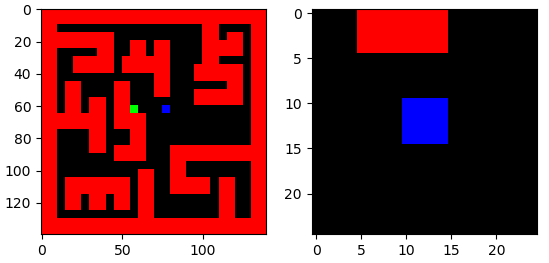
\includegraphics[width=0.7\textwidth]{maze}
  \caption{The agent (blue) has to find the target (green) in the maze (left,
    walls in red). It is only provided a history of partial observations
    (right).}
  \label{fig:maze}
\end{figure}

At each time step the agent has to decide the direction (up, right, down, left)
for the following discrete move by the current and some preceding pob.
Pob and optimal directions for training and validation are generated via
A-Star-Algorithm.
For testing the agent has to maximize the number of successful runs.
A run is only successful if the agent finds the target in a limited number of
time.
In \autoref{sec:generalization} we investigate the influence of changing target position, map,
history and pob on the test performance.

\section{Implementation}
\textbf{TODO: How well does your agent perform from the local view ?}
\textbf{TODO: What happens if you increase the history length for the views or make the
view larger ?}
\section{Generalization}\label{sec:generalization}

\begin{figure}
    \centering
    \begin{subfigure}[b]{0.3\textwidth}
        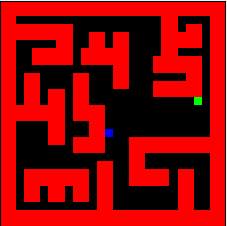
\includegraphics[width=\textwidth]{random_target}
        \caption{randomized target position}
        \label{fig:randomtargetmaze}
    \end{subfigure}
    ~ %add desired spacing between images, e. g. ~, \quad, \qquad, \hfill etc.
      %(or a blank line to force the subfigure onto a new line)
    \begin{subfigure}[b]{0.3\textwidth}
        %\includegraphics[width=\textwidth]{}
        \caption{slightly modified maze}
        \label{fig:othermaze}
    \end{subfigure}
    \caption{The agent tries using the way it learned while training to a fixed
      position where it expects the target. Any changes there results in
      the agent to only move back and forth.}\label{fig:generalization}
\end{figure}

\subsection{Target location}
\textbf{TODO: What happens if you change the target location after training (you can
change it in utils.py) ?}
\subsection{Map}
\textbf{TODO: What happens if you change the map after training (how well does your
agent generalize) ?}
\subsection{Proposal}
\textbf{TODO: Can you think of ways to make the agent generalize across target locations
different maps ?}

\textbf{TODO: For bonus points: test one of these ideas.}

% \begin{thebibliography}{99}
% \end{thebibliography}

\end{document}
